\chapter{Integración en sistemas CI/CD}\label{sec:cicd}

\paragraph{}Cuando hablamos de sistemas \gls{CI/CD} nos solemos referir a todos aquellos
servidores, servicios y máquinas; ya sean \gls{on premises} o en cloud, que posibilitan
el desarrollo centralizado, el control de versiones, el aseguramiento de la calidad
y la entrega continua.

\begin{figure}[H]
    \centering
    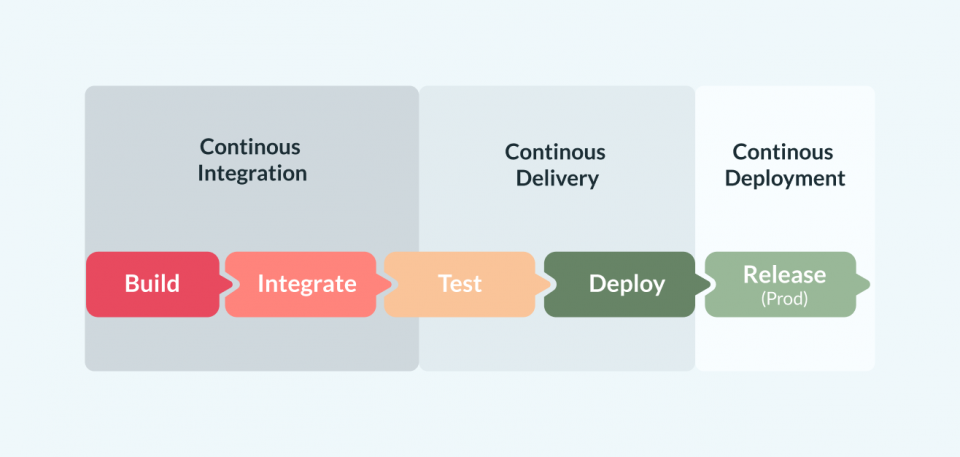
\includegraphics[width=0.75\textwidth]{imgs/cicd}
    \caption{Esquemas de estrategia CI/CD.}
    \label{imgs:cicd}
\end{figure}


\paragraph{}\textbf{Nota: }\emph{Cómo entrar en detalle en estos apartados sería extender
demasiado el alcance que se prentende en este trabajo, este capítulo se va a limitar a
describir la relación del entorno de desarrollo con los sistemas \gls{CI/CD}. Cualquier
arquitectura de la infraestructura es pura expeculación y no será probada a nivel práctico.}

\section{Control de versiones}

\paragraph{}El control de versiones en este entorno de desarrollo se realiza mediante
\gls{git}. \Gls{git} es una herramienta de control de versiones gratuita, multiplataforma que
es muy popular, tanto que incluso podría empezar a considerarse un estandar. Populares
servicios de repositorios online, como \href{github.com}{github} o \href{gitlab.com}{gitlab}
funcionan con este sistema. Para este proyecto, se ha elegido \href{github.com}{github}
por su popularidad. Ya que al ser código abierto, esto facilita que más desarrolladores
encuentren el proyecto e incluso quieran colaborar para hacer sus aportaciones. Además,
github permite aplicar la política de branching GitHub-Flow, la cual explicaremos más
adelante en detalle.

\paragraph{}En mi experiencia laboral, he utilizado \gls{git} en repositorios compartidos
por más de mil desarrolladores y \gls{git} facilita la gestión del control de versión.
Obviamente, en casos tan ``extremos'' como el mencionado, existen carencias que no
resuelve la propia herramienta, y que han de ser solventados mediante la implantación
de protocolos internos y patrones de branching.

\paragraph{}Algunos de los patrones más utilizados son: patrón release-ready mainline,
hot-fix branch, feature branch, release branch o production branch. Estos patrones deben
ser implementados en función de la naturaleza del proyecto, de la cantidad de cambios que
sufre el código, la metodología de desarrollo de la empresa, de la relación con el
cliente, etc.

\subsection{Ciclo de vida del desarrollo software}

\paragraph{}Como se puede apreciar en la imagen \ref{imgs:recipe-rpi-weather-1} cada
vez que se haga un \gls{fetch} de Rpi Weather, se va a descargar lo último que haya en la
rama principal. Esto tiene unas consecuencias inmediatas. La rama principal debe contener
en todo momento código funcional dispuesto a ser entregado y que pase todas las pruebas
necesarias. En un entorno real, lo más conveniente sería fijar la referencia de una recipe,
o bien a un \emph{tag} o \emph{commit} concretos o bien a una rama de release. Pero para
nuestro ejemplo, vamos a considerar la rama \emph{main} como una rama de release.

\begin{figure}[H]
    \centering
    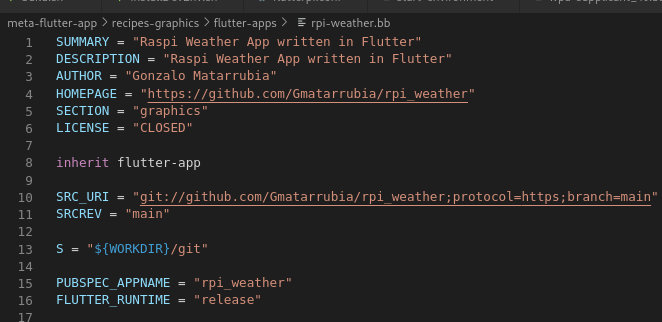
\includegraphics[width=0.90\textwidth]{imgs/rpi-weather-recipe}
    \caption[Detale recipe de Rpi Weahter]{Detalle de la recipe de Rpi Weather.}
    \label{imgs:recipe-rpi-weather-1}
\end{figure}

\paragraph{}Yocto admite tener tanto fuentes locales, como fuentes en servidores. Por
eso mismo, para el desarrollo de la aplicación flutter se propone el uso de los
siguiente patrones de branching, explicando sus fundamentos.

\paragraph{Política de branching GitHub-Flow:} Está política de branching agrupa unos
cuantos patrones que adapta a su plataforma online. GitHub-Flow está orientado a proyectos
con una sola versión en producción y una alta frecuencia de integraciones en la rama
principal, la cual será una \emph{Release-Ready Mainline}\ref{sec:release-ready}. En
principio las release branch no son necesarias, ni tampoco las Hotfix branch, éstas
últimas existiran pero no será diferentes de una feature branch normal. Nadie trabajará
en la rama principal, cada característica/función/mejora debe hacerse en una \emph{feature
branch}. Dicha función o mejora debe estar acotada y una vez terminada, se hará una
\emph{pre-integration review}, es decir que se revisarán los cambios que se quieren
introducir en la rama principal. Una vez revisados y aprobados los cambios, es común
que se realice una serie de comprobaciones automáticas y en caso de éxito, se integren
los cambios en la rama principal. Las comprobaciones automáticas pueden incluir, análisis
dinámico y/o estático de código, test unitarios, test de integración, compilación, etc.
En Github, esta revisión tiene su propia herramienta llamada \emph{Pull Request}.

\begin{figure}[H]
    \centering
    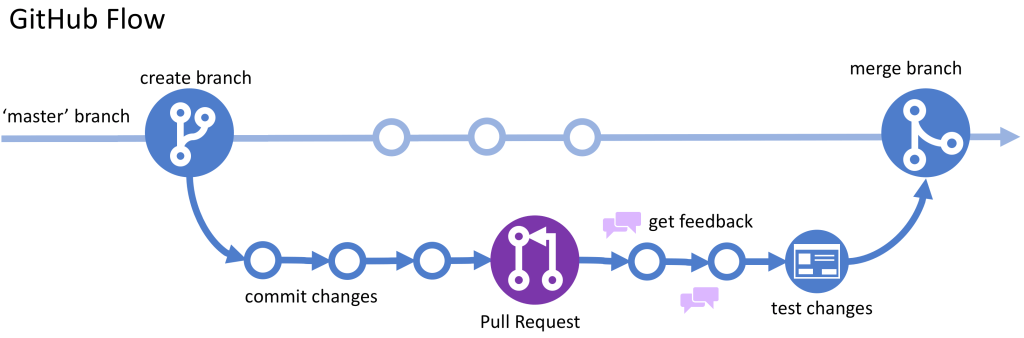
\includegraphics[width=0.85\textwidth]{imgs/github-flow}
    \caption{Esquema de una rama en Github Flow}
    \label{imgs:github-flow}
\end{figure}

\paragraph{Patrón Release-ready Mainline:}\label{sec:release-ready}

\paragraph{}Como su propio nombre indica, este patrón de branching nos indica que cada
\emph{commit} hecho en la línea principal o \emph{mainline} debe poder ser liberado a
producción. No obstante, conviene aclarar que el hecho de que pueda ser ``liberable'',
no significa que tenga que serlo. Dependera de si la empresa practica el \emph{continuous
deployment} o \emph{continous delivery}, en este último caso serán las decisiones de
negocio las que decidirán que versión desplegar a producción de entre todas las versiones.


\paragraph{Patrón Feature branch:} Una feature branch se utilizará para conjuntos de
cambios que tengan una relación lógica. Los objetivos de una feature branch, deben ser
medibles y finitos. De menera que cada característica nueva del programa, cada bug, etc
esté en su propia rama exclusiva.

\subsection{Infraestructura}

\paragraph{}Normalmente, los sistemas de control de versiones están ``supervisados''
por equipos de compilación, analizadores estáticos y dinámicos, despligue de artefactos,
etc. Es decir, que existe una infraestructura que trabaja de forma automatizada con
nuestro código y los cambios que le introducimos. Esta infraestructura puede estar
en local, \gls{on premises} o en cloud. Lo único que cambia en cada caso es la hubicación
física del \emph{hardware}, así como la responsabilidad de mantener el servicio.

\paragraph{}Para asegurar la mantenibilidad de esta infraestructura, así como para aplicar
las mismas técnicas de desarrollado que se hacen con el código se llevan a cabo descripciones
de \glsplural{pipeline} en lo que se conoce como \gls{IaaC}. De esta manera, el desarrollo
del entorno de desarrollo, valga la redundancia, y sus dependencias puede ser desarrollado
y administrado a la vez y de igual manera que el propio código que contiene.

\paragraph{}Las \glsplural{pipeline} pueden estar contenidas en el propio repositorio
junto al código, lo cual traza una estrategia de infraestructura orientada al proyecto,
o puede estar en un repositorio a parte de manera que pueda ser utilizada en común con
otro proyecto.

\paragraph{}Los \glsplural{pipeline} sólo definen las acciones a realizar en la infraestructura
en determinados eventos, pero la propia definición de la infraestructura también puede
estar definida en código. En nuestro proyecto, los repositorios están pensados para
integrarse en una infraestructura \gls{IaaC} mediante Ansible\ref{sec:ansible}. En este
proyecto, por su alcance, se han definido unos \emph{playbooks} o unidades de configuración,
implementación y aprovisionamiento reutilizables, en las que deben ser lanzados de forma
local. De esta forma, no habría mucha diferencia con un script normal, más haya de la
sintaxis y el uso de ciertos módulos pre-integrados. En cambio, aplicado Ansible a toda
la infraestructura podría facilitar la preparación de los equipos dónde se a desarrollar
los diferentes entornos, así como las máquinas donde se van a procesar los entornos.

\paragraph{}Con Ansible, por ejemplo, sería muy fácil crear dispositivos nuevos para
nuevos trabajadores que fueran a utilizar los diferentes entornos, aplicando de manera
automática los \emph{playbooks} necesarios en cada caso. Incluso si se realizara un
cambio de requisito y/o entorno, con Ansible podría administrarse todos los equipos,
por lotes y de forma automática y remota.

\section{QA}

\paragraph{}Los mecanismos de infraestructura recomendados para cada entorno cambian.
Como no hay muchas herramientas externas de yocto que permitan hacer un análisis más
avanzado del que hace el propio yocto al generarse, para ese entorno uno o varios nodos
que tengan un servicio de generación centralizado sería suficiente. Incluso se podría
tener un entorno de pre-producción y comprobar la integración hardware como parte del
proceso de \emph{quality assurance}. Los nodos de generación automática podrían utilizar
Jenkins para esta tarea, o bien un alternativa sería utilizar los recursos de GitHub
Actions. Quizás el factor más importante en este caso sería si esta parte de la
infraestructura se quiere hacer el could o \gls{on-premises}. En ambos casos, se
describiría la una \gls{pipeline} en un archivo específico en el propio repositorio de
código.

\begin{figure}[H]
    \centering
    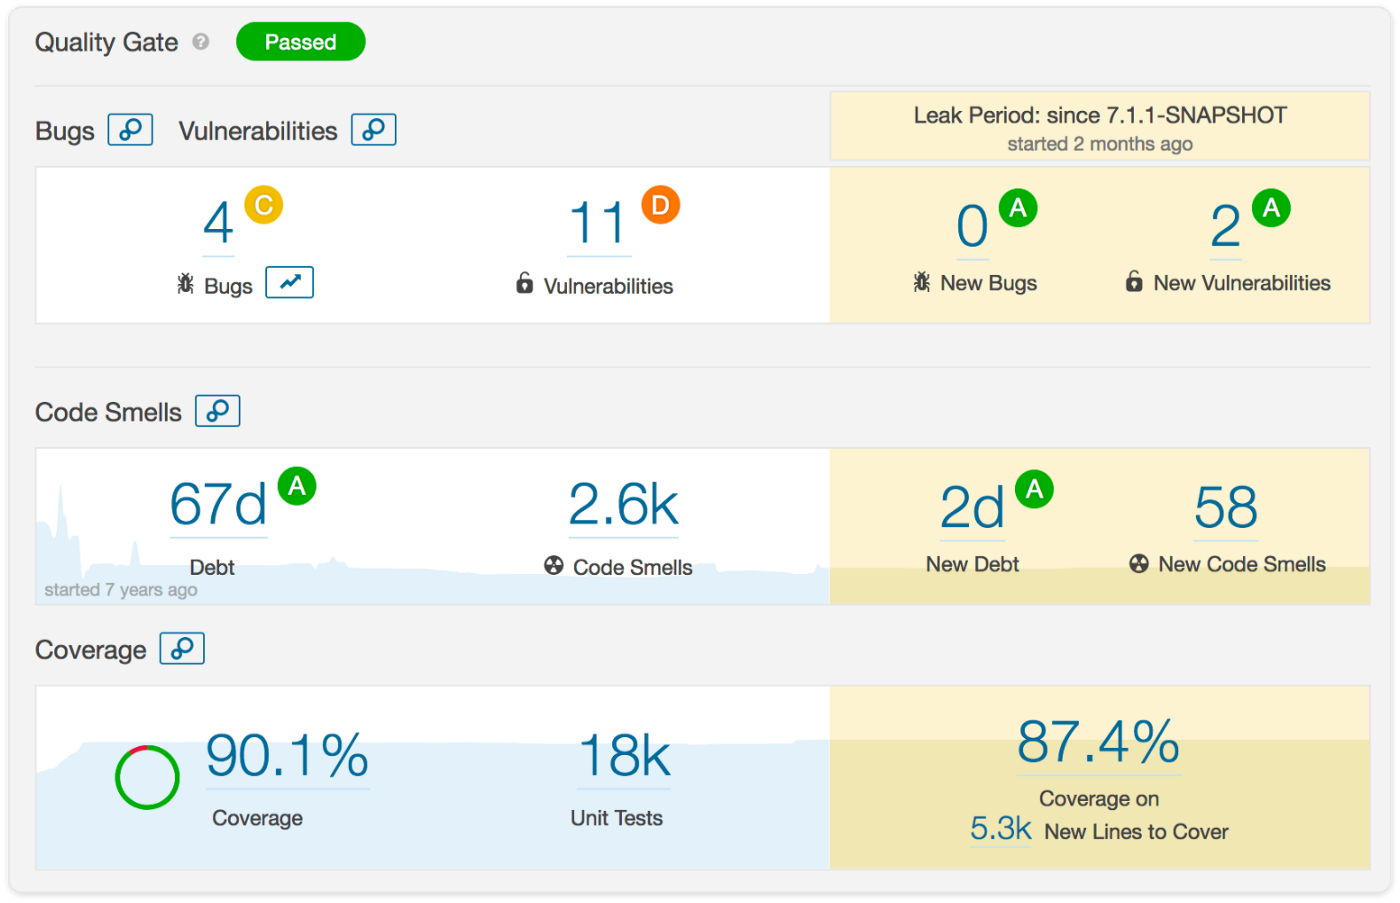
\includegraphics[width=0.85\textwidth]{imgs/sonarqube}
    \caption{Panel principal de Sonarqube}
    \label{imgs:sonarqube}
\end{figure}

\paragraph{}El entorno Flutter admite más variaciones en cuanto a el uso de infraestructura
para gestionar el \emph{quality assurance}. Puede haber nodos de compilación automática,
pero también nodos de análisis de código y ejecución de test. Por ejemplo, se puede
utilizar una instancia de Sonarqube, para obtener resultados acerca de la calidad y del
código, abarcando desde el uso del \gls{coding standard} hasta la deteción de vulnerabilidades.

\paragraph{}El QA siempre tiene una componente subjetiva y que difícilmente se puede
automatizar, así además de medios, para garantizar una buena calidad se necesitan
trabajadores cualificados para dicha tarea.

\section{Entrega continua}

\paragraph{}Hay varias soluciones comerciales que se integran con Yocto para realizar
la entrega continua, tanto para la actualización de la aplicación Flutter dentro del
sistema como para realizar un \emph{full-upgrade} a todo el firmware. En el caso de
querer realizar las actualizaciones \gls{OTA} solo para la aplicación flutter se tienen
más alternativas, ya que podríamos modificar el sistema operativo para instalar cualquier
servicio que aporte esta utilidad. En el caso de querer realizar un \emph{full-upgrade}
es necesario contar con determinadas características del hardware.

\paragraph{}Las estategias más frecuentes para realizar un ``\emph{full-upgrade}'' son:
\begin{itemize}
    \item Disco de arranque de actualización/recuperación.
    \item Hipervisor.
        \subitem Tipo 1 o baremetal.
        \subitem Tipo 2, con un sistema operativo \emph{host} y otro \emph{guest}.
\end{itemize}

\begin{figure}[H]
    \centering
    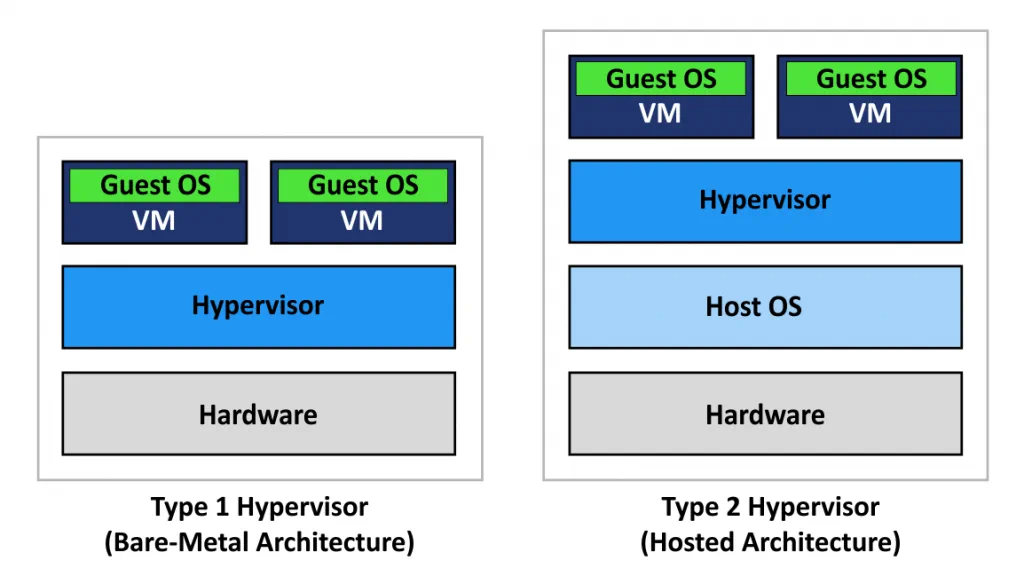
\includegraphics[width=0.75\textwidth]{imgs/hypervisor}
    \caption{Esquemas de los tipos de hipervisor.}
    \label{imgs:hipervisor}
\end{figure}

\paragraph{}En nuestro caso, al basarnos en un hardware Raspberry Pi, dependemos del
modelo para encontrar casos de éxito basados en hipervisores. Entonces el enfoque con
más sentido sería crear una partición de rescate autoarrancable de solo lectura y que
permitiera actualiar la otra partición. Este mecanismo habría que diseñarlo y desarrollarlo
en Yocto.

%las referencias a artculos se ponen con \cite,
%las referencias a imgenes \ref,
%las referencias a glosario \gls,
%y las referencias a ecuaciones \eqref
